%
% LaTeX report template 
%

% This is a comment: in LaTeX everything that in a line comes
% after a "%" symbol is treated as comment

\documentclass[11pt, a4paper]{article}
\usepackage{graphicx}
\usepackage{amsmath}
\usepackage{listings}
\usepackage{url}
\usepackage{float}
\usepackage{xcolor}

\definecolor{codegreen}{rgb}{0,0.6,0}
\definecolor{codegray}{rgb}{0.5,0.5,0.5}
\definecolor{codepurple}{rgb}{0.58,0,0.82}
\definecolor{backcolour}{rgb}{0.95,0.95,0.92}

\lstdefinestyle{mystyle}{
    backgroundcolor=\color{backcolour},   
    commentstyle=\color{codegreen},
    keywordstyle=\color{magenta},
    numberstyle=\tiny\color{codegray},
    stringstyle=\color{codepurple},
    basicstyle=\ttfamily\footnotesize,
    breakatwhitespace=false,         
    breaklines=true,                 
    captionpos=b,                    
    keepspaces=true,                 
    numbers=left,                    
    numbersep=5pt,                  
    showspaces=false,                
    showstringspaces=false,
    showtabs=false,                  
    tabsize=2
}

\lstset{style=mystyle}

\title{EE2703: Applied Programming Lab \\ Assignment No 5: The Resistor Problem} % Title

\author{Ishaan Agarwal \\ EE20B046} % Author name

\date{\today} % Date for the report
\begin{document}		
		
\maketitle % Insert the title, author and date

\section{Introduction}
%Create new section;it is autonumbered
The aim of this assignment is to obtain the solution to the potential in a region subject to the given constraints by solving \textit{Laplace's} equation in two-dimensions.\\
\textit{Laplace's} equation in two-dimensions can be written as (in Cartesian coordinates):
\[\frac{\partial^2 \phi}{\partial x^2} + \frac{\partial^2 \phi}{\partial y^2} = 0\] 
Using suitable approximations for a discrete point grid, we get 
\[\phi_{i,j} = \frac{\phi_{i, j-1} + \phi_{i-1, j} + \phi_{i, j+1} + \phi_{i+1, j}}{4}\]

The physical significance of this would be that the potential at any point is the sum of the values at it's nearest neighbouring points. We have basically used this equation to solve the given problem by updating $\phi$ over many iterations till it converges within an acceptable error. 


\section{Solution}
\subsection{The potential solution using \textit{Laplace's} equation}
As mentioned earlier, we use the updation formula in multiple iterations and take care of the boundary conditions in each step as well. This is done using:
\\

\begin{lstlisting}[language = Python]
#creating the potential grid
phi = np.zeros((Ny,Nx))

#creating position vectors
x = np.linspace(-((Nx-1)//2), Nx//2, Nx) # since phi uses integral indices, we cannot just do -Nx/2,Nx/2
y = np.linspace(-((Ny-1)//2), Ny//2, Ny) 

X,Y = np.meshgrid(x,y)

#using numpy.where() to find the points within the radius
ii = np.where(X**2 + Y**2 <= radius**2)

#set potential at those points as one
phi[ii] = 1

#contour plot of phi versus x and y
plt.contourf(x, y, phi)
plt.colorbar()
plt.scatter(X[ii], Y[ii], c='r', marker = 'o', label = 'points within radius (V=1V)')
plt.plot(0,0, 'bo', label = 'center')
plt.xlabel('x')
plt.ylabel('y')
plt.title('Contour plot of Potential')
plt.legend()
plt.show()

def update_phi(phi, oldphi): #update phi using given formula
    phi[1:-1, 1:-1] = (oldphi[0:-2, 1:-1] + oldphi[2:, 1:-1] + oldphi[1:-1, 0:-2] + oldphi[1:-1, 2:])/4
    return phi

def boundary_conditions(phi): #boundary conditions
    phi[1:-1, 0] = phi[1:-1, 1]
    phi[1:-1, -1] = phi[1:-1, -2]
    phi[0, 1:-1] = phi[1, 1:-1]
    phi[-1, 1:-1] = 0
    phi[ii] = 1
    return phi
\end{lstlisting}

\begin{figure}[H]
     \centering
     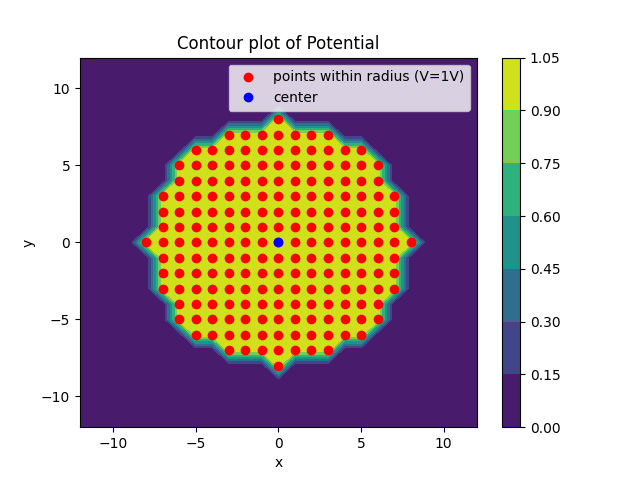
\includegraphics[scale=0.8]{Figure_1.png}
\end{figure}





\subsection{Error in estimations}
In every iteration, we keep track of the error by finding the maximum value of the error between the new phi matrix elements and the old phi matrix elements. 
\\
\begin{lstlisting}[language = Python]
#keeping track of errors
errors = np.zeros(Niter)

for k in range(Niter):
    oldphi = np.copy(phi)   #making a copy of phi
    phi = update_phi(phi, oldphi) #updating phi
    phi = boundary_conditions(phi) #applying boundary conditions
    errors[k] = (np.abs(phi - oldphi).max()) #appending error

#plotting the errors
plt.plot(range(Niter)[::50], errors[::50], 'ro--', label = 'error')
plt.xlabel('iteration')
plt.ylabel('error')
plt.title('Error vs. iteration')
plt.legend()
plt.show()

#plotting the errors of every 50th iteration on a semilogy plot
plt.semilogy(range(Niter)[::50], errors[::50], 'ro--', label = 'error')
plt.xlabel('iteration')
plt.ylabel('error')
plt.title('Error vs iteration on a semilogy scale')
plt.legend()
plt.show()

#plotting the errors on a log log plot
plt.loglog(range(Niter)[::50], errors[::50], 'ro--', label = 'error')
plt.xlabel('iteration')
plt.ylabel('error')
plt.title('Error vs iteration on a loglog scale')
plt.legend()
plt.show()


\end{lstlisting}

These errors are the plotted against the number of iterations on a linear, semilogy and a loglog scale.

\begin{figure}[H]
     \centering
     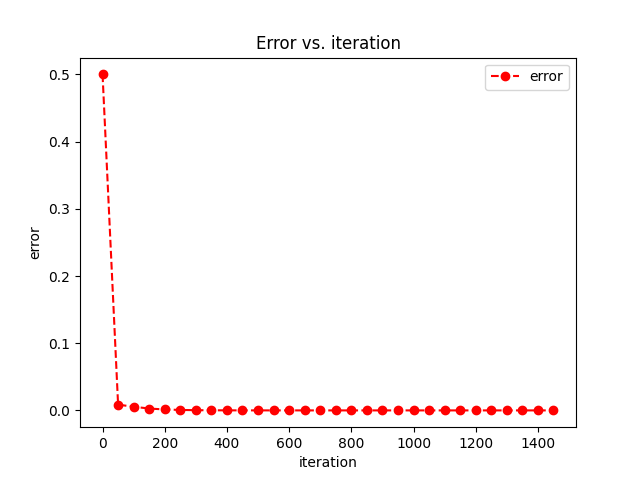
\includegraphics[scale=0.8]{Figure_2.png}
\end{figure}

\begin{figure}[H]
     \centering
     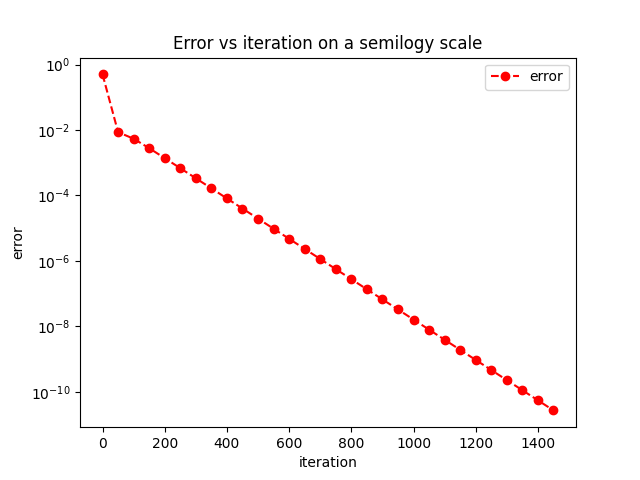
\includegraphics[scale=0.8]{Figure_3.png}
\end{figure}

\begin{figure}[H]
     \centering
     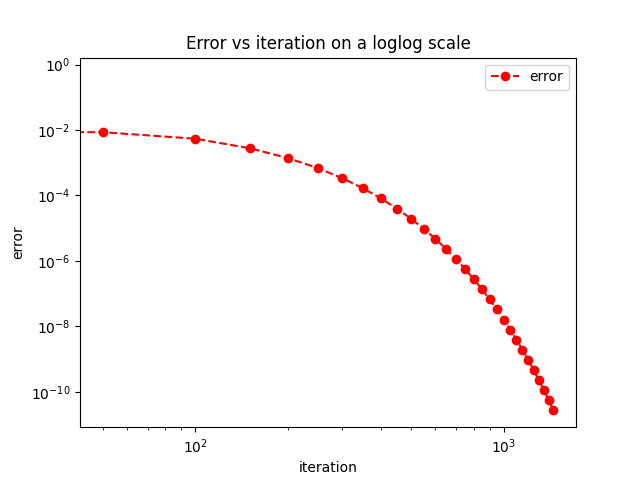
\includegraphics[scale=0.8]{Figure_4.png}
\end{figure}

We observe that the error vs number of iterations on a semilogy scale is nearly linear and thus we conclude that the error vs number of iterations might be a decaying exponential.


\subsection{Least Squares Fit}
Now, we attempt to extract the dependence of error on the number of iterations, by fitting an exponential to the plotted curve. This can be accomplished by creating a linear equation and then using \texttt{np.linalg.lstsq()}. 

\[y = Ae^{Bx} \]
\[\log{y} = \log{A} + Bx\]
The above equation is linear, and thus \texttt{np.linalg.lstsq()} can be used to find the corresponding coefficients. \\
The corresponding code is:
\\
\begin{lstlisting}[language = Python]
#finding the least squares fit using lstsq
def error_fit(x, y):
    a = np.vstack([x, np.ones(len(x))]).T
    B, logA = np.linalg.lstsq(a, y)[0]
    return B, np.exp(logA)

#fitting an exponential
def exp_fit(x, A, B):
    return A*np.exp(B*x)

errors[errors == 0] = np.min(errors[errors != 0])*10**(-20) #ensuring there are no zero values before taking log

#finding fit 1
x1 = range(Niter)
y1 = np.log(errors)
B1, A1 = error_fit(x1, y1)
plt.semilogy(x1[::50], exp_fit(x1[::50], A1, B1), 'ro--', label = 'Fit1', ms = 5, alpha = 0.5)

#finding fit 2
x2 = range(500, Niter)
y2 = np.log(errors[500:])
B2, A2 = error_fit(x2, y2)
plt.semilogy(x2[::50], exp_fit(x2[::50], A2, B2), 'bo--', label = 'Fit2', ms = 5, alpha = 0.5)

#original
plt.semilogy(range(Niter)[::50], errors[::50], 'ko--', label = 'Original errors', ms = 3, linewidth = 3, alpha = 0.8)
plt.title('Fitting using least squares')
plt.legend()
plt.show()
\end{lstlisting}

After fitting, we plot the \textit{fit$1$}, \textit{fit$2$} approximations for every 50th element and the original error on the same plot.

\begin{figure}[H]
     \centering
     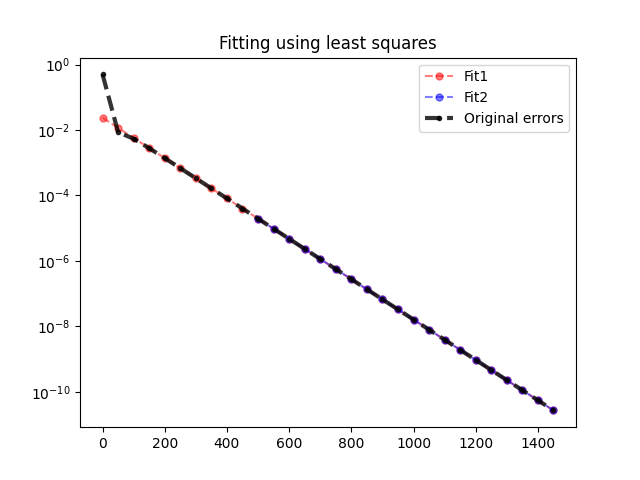
\includegraphics[scale=0.8]{Figure_5.png}
\end{figure}

As we see, both the fits are very close to the original graph, on zooming in, we notice that the \textit{fit$2$} graph is much more closer to the original graph than \textit{fit$1$}, this is because the magnitude of errors in the beginning is much larger, thus causing a larger error, whereas \textit{fit$2$} only takes into account, the iterations after 500, where the errors are much smaller and thus the fit is more accurate. 


\subsection{Stopping condition}
The upper bound for the error estimated with each iteration is given by:
\[Error = -\frac{A}{B}*\exp(B(N+0.5))\]
We thus plot this upper bound of the errors vs the number of iterations on a semilogy plot.
\\
\begin{lstlisting}[language = Python]

#upper bound of errors
def max_error(A, B, N):
    return -A*(np.exp(B*(N+0.5)))/B

#plotting the upper bounds of the errors
plt.semilogy(range(Niter)[::50], max_error(A1, B1, np.array(range(Niter)[::50])), 'ro--', label = 'Upper bound of errors')
plt.title('Upper bound of errors')
plt.legend()
plt.show()

\end{lstlisting}

The corresponding plots are:

\begin{figure}[H]
     \centering
     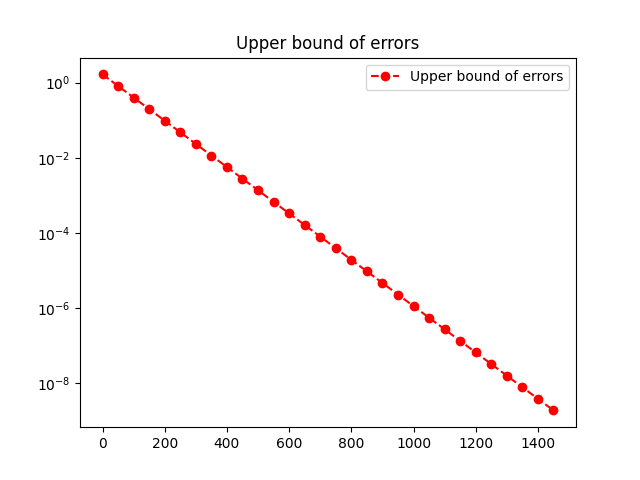
\includegraphics[scale=0.8]{Figure_6.png}
\end{figure}


\subsection{Surface Plot of potential}
After running the algorithm using the suitable conditions, we plot our final potential grid on a 3-D surface plot for better visualisation using the \texttt{plot\_surface} function.
\\

\begin{lstlisting}[language = Python]
#surface plot of potential
fig = plt.figure()
ax = p3.Axes3D(fig)
surf_plot = ax.plot_surface(X, Y, phi, rstride = 1, cstride = 1, cmap = 'jet')
fig.colorbar(surf_plot)
ax.set_xlabel('y')
ax.set_ylabel('x')
ax.set_zlabel('potential')
ax.set_title('Surface plot of Potential')
plt.show()
\end{lstlisting}

\begin{figure}[H]
     \centering
     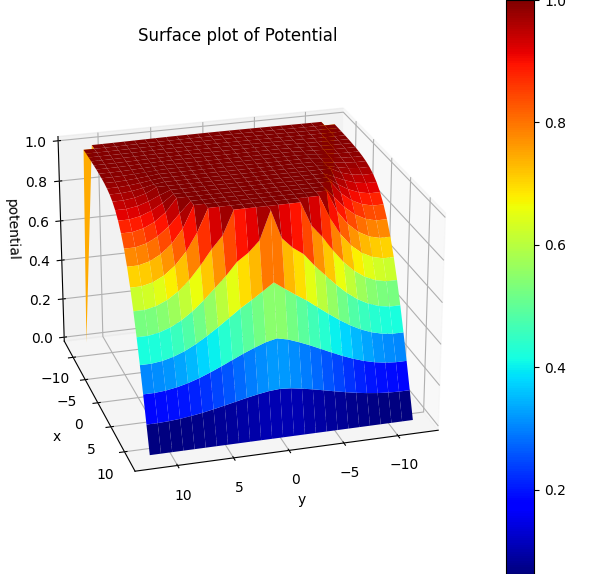
\includegraphics[scale=0.8]{Figure_7.png}
\end{figure}

\subsection{Contour Plot of potential}
We now plot the contourf plot for the potential after the algorithm is run using the \texttt{plt.contourf} function.
\\

\begin{lstlisting}[language = Python]
#contourf plot of potential
plt.contourf(x, -y, phi)
plt.colorbar()
plt.scatter(X[ii], Y[ii], c = 'r', marker = 'o', label = 'points within radius (V=1V)')
plt.plot(0,0, 'bo', label = 'center')
plt.xlabel('x')
plt.ylabel('y')
plt.title('Contour plot of Potential')
plt.legend()
plt.show()
\end{lstlisting}

\begin{figure}[H]
     \centering
     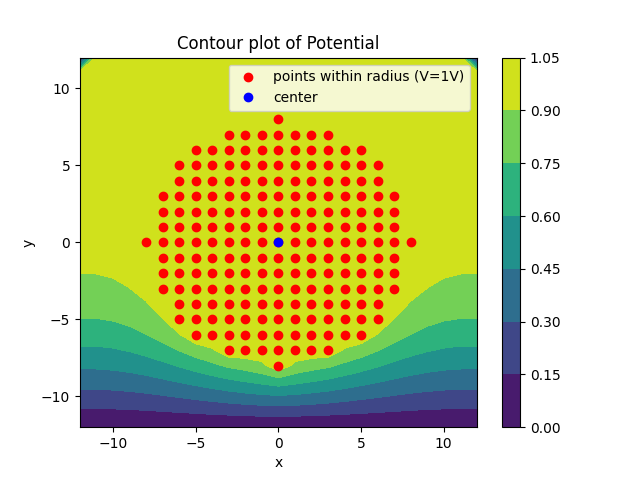
\includegraphics[scale=0.8]{Figure_8.png}
\end{figure}

\subsection{Vector Plot of Currents}
Next, we try to find the currents in the system. We know that, the currents in the system are given as:
\[j_x = - \frac{\partial \phi}{\partial x}\]
\[j_y = - \frac{\partial \phi}{\partial y}\]

For our problem, this numerically translates to:

\[j_{x,ij} = \frac{1}{2}(\phi_{i,j-1} - \phi_{i,j+1})\]
\[j_{y,ij} = \frac{1}{2}(\phi_{i-1,j} - \phi_{i+1,j})\]

We then plot these current densities using the \texttt{plt.quiver()} function.
\\
\begin{lstlisting}[language = Python]

#vector plot of currents
#creating jx and jy of same dimensions as phi
jx = np.zeros(phi.shape)
jy = np.zeros(phi.shape)

jx[:, 1:-1] = (phi[:, 0:-2] - phi[:, 2:])/2
jy[1:-1, :] = (- phi[0:-2, :] + phi[2:, :])/2

#plotting vector plot using quiver
plt.quiver(x, y, jx[::-1,:], jy[::-1,:], scale = 4)
plt.scatter(X[ii], Y[ii], c = 'r', marker = 'o', label = 'points within radius (V=1V)')
plt.plot(0,0, 'bo', label = 'center')
plt.xlabel('x')
plt.ylabel('y')
plt.title('Vector plot of currents')
plt.legend()
plt.show()

\end{lstlisting}

\begin{figure}[H]
     \centering
     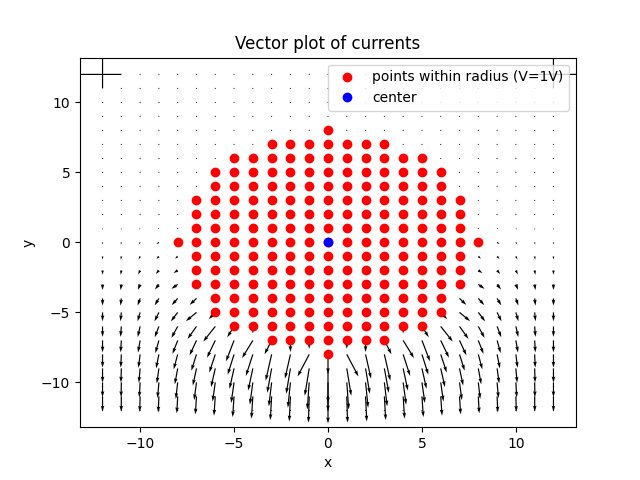
\includegraphics[scale=0.8]{Figure_9.png}
\end{figure}

We thus notice that very little current flows through the top portion of the wire. This is because the lower surface is grounded (kept at zero potential), thus the easiest way for charge carriers to flow from the electrode would be directly through the lower half of the wire and not through the longer more resistance path through the upper half of the wire. 


\section{Conclusion}
We thus have solved the \textit{Laplace's} differential equation in a numerical fashion using gridpoints. The error is seen to be decaying almost exponentially and thus an exponential fit was found which fit the error curve almost exactly. From the current density plots, we notice that most of the current only flows in the bottom half of the wire. Thus, we expect the bottom part of the wire to get heated the most due to Ohmic losses.


\end{document}



 